\documentclass[../main.tex]{subfiles}
\begin{document}

\subsection{Project Background}
\label{sec:project-background}

In recent years, \gls{dl} has significantly improved the
performance of computer vision systems in image classification, object
detection and segmentation tasks.
\gls{gans} in particular have revolutionized generative tasks like image synthesis
and image-to-image translation. Image-to-image translation is the
problem where we have a source image and we want to generate an image
based on the source but with different characteristics.

In this work, the idea of image-to-image translation is applied
to the transformation of \gls{cm} histological images into \gls{he} appearance.

\subsubsection{Confocal microscopy}
Ex vivo\footnote{Ex vivo means that which takes place outside an organism.
In science, ex vivo refers to experimentation or measurements done in or on
tissue from an organism in an external environment with minimal alteration
of natural conditions.} confocal scanning laser microscopy can potentially
accelerate Mohs surgery\footnote{Mohs micrographic surgery is considered the
most effective technique for treating many basal cell carcinomas (BCCs) and
squamous cell carcinomas (SCCs), the two most common types of skin cancer.
The procedure is done in stages, including lab work, while the patient waits.
This allows the removal of all cancerous cells for the highest cure rate
while sparing healthy tissue and leaving the smallest possible scar.}
in rapidly detecting carcinomas without conventional frozen histopathology.

\gls{cm} has enabled rapid evaluation of tissue samples
directly in the surgery room significantly reducing the time of complex
surgical operations in skin cancer (\cite{Cinotti2018}),
but the output largely differs from the standard \gls{he} slides that
pathologists typically use to analyze tissue samples.

\gls{cm} is an optical imaging technique for increasing optical resolution
and contrast of a micrograph by means of using a spatial pinhole to block
out-of-focus light in image formation. With it, technician are able to slice
thin optical sections out of thick fluorescent specimens, view specimens
in planes tilted to the line of sight, penetrate deep into light-scattering
tissues, obtain 3D views at very high resolution... (\cite{Inoue2006})
Two different \gls{cm} modes exist, \gls{rcm} displays the backscattering signal
of naturally occurring skin components, whereas \gls{fcm} provides contrast
by using an applied fluorescent dye (\cite{Skvara2012}).

\begin{figure}[h]
\centering
\begin{subfigure}{.5\textwidth}
  \centering
  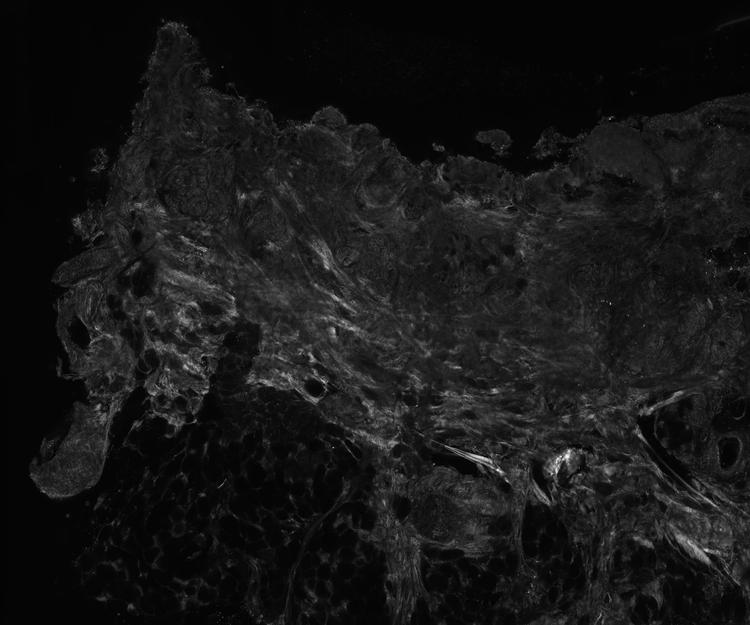
\includegraphics[width=.8\linewidth]{R_crop_thumbnail}
  \label{fig:R-example}
\end{subfigure}%
\begin{subfigure}{.5\textwidth}
  \centering
  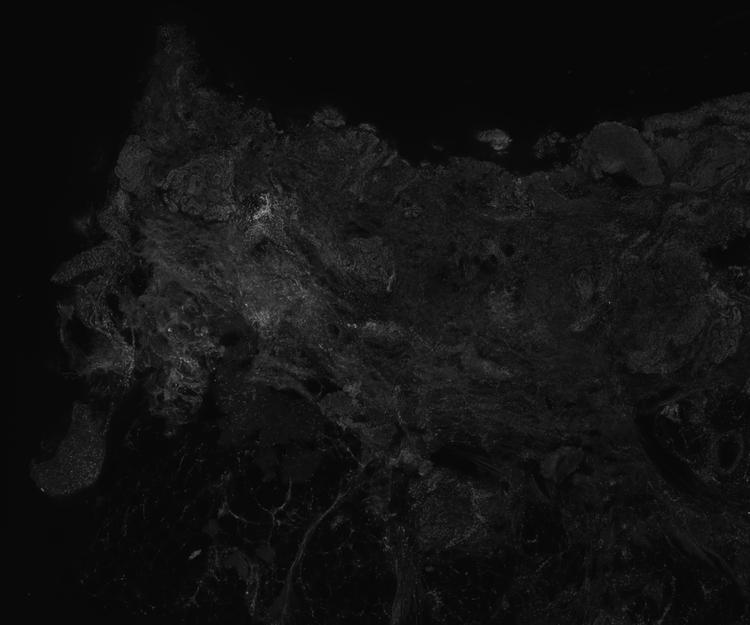
\includegraphics[width=.8\linewidth]{F_crop_thumbnail}
  \label{fig:F-example}
\end{subfigure}
\caption{Example of a CM micrograph of a skin tissue.
reflectance mode on the left and fluorescence mode on the right}
\label{fig:CM-example}
\end{figure}

\subsection{Problem statement}
\label{sec:problem-statement}
% In the previous work, a \gls{dl} technique is proposed to combine
% the two modes of the \gls{cm} into a H\&E-like image to facilitate their
% interpretation by untrained pathologists and surgeons.

% The initial chosen architectures are: a \gls{cnn} with a multiplicative
% residual connection to reduce the noise and then a \gls{cyclegan} to combine
% the two CM modes into a digitally stained slide.

% The current model has room for improvements: the despeckling neural
% network sometimes produces undesired artifacts and de stain generative
% network can create or eliminate structures on the output image. This
% project will focus on understanding why this happens and will try to
% solve this problems.

% In contrast to the work by Gareau et. al...
% data-driven approach...
\lipsum

\subsection{Methods and procedures}
\label{sec:methods-and-procedures}
This project was carried out at the Image and Video Processing Group (GPI) research
group from the Signal Theory and Communications Department (TSC) at the Universitat
Politecnica de Catalunya (UPC) in collaboration with the Dermatology Department from
the Hospital Clínic de Barcelona.

The work presented in this thesis is the natural continuation of the work presented
in \cite{Combalia2019}...

\subsection{Document Structure}
\lipsum

\end{document}
